% Appendix Template

\chapter{Results of experiment 2.2} % Main appendix title

\label{Appendix2-2} % Change X to a consecutive letter; for referencing this appendix elsewhere, use \ref{AppendixX}

\begin{figure}[th]
\centering
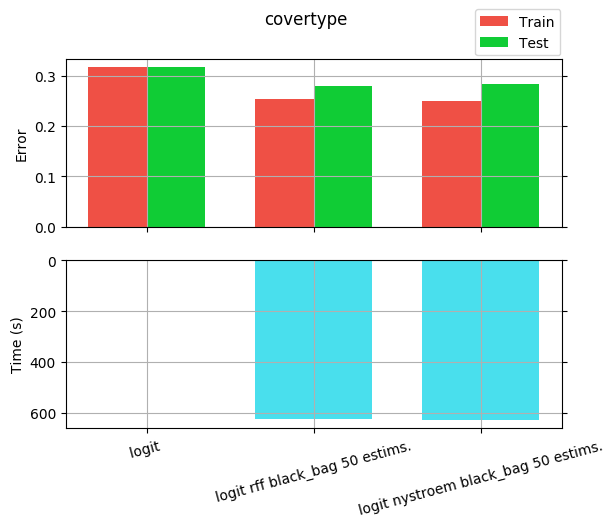
\includegraphics[scale=\imgscale]{Figures/2_2/covertype}
\decoRule
\caption[2.2 covertype]{Logistic Regression with Black Bag model}
\label{fig:2_2_covertype}
\end{figure}

\begin{figure}[th]
\centering
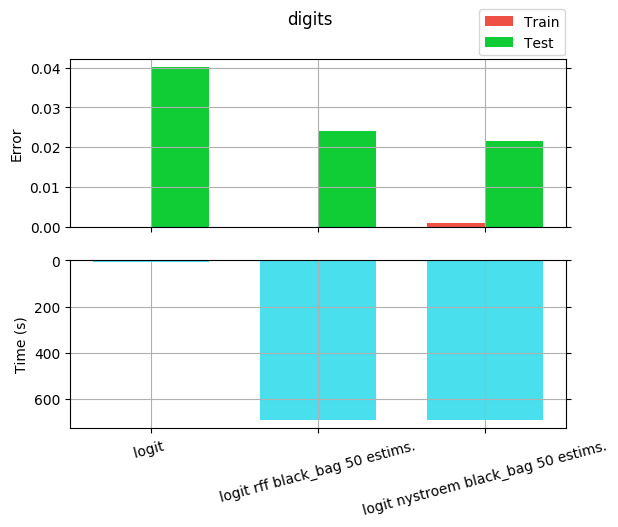
\includegraphics[scale=\imgscale]{Figures/2_2/digits}
\decoRule
\caption[2.2 digits]{Logistic Regression with Black Bag model}
\label{fig:2_2_digits}
\end{figure}

\begin{figure}[th]
\centering
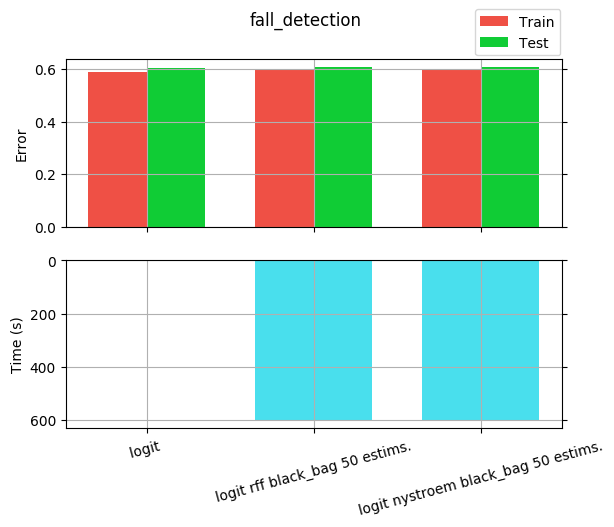
\includegraphics[scale=\imgscale]{Figures/2_2/fall_detection}
\decoRule
\caption[2.2 fall\tu detection]{Logistic Regression with Black Bag model}
\label{fig:2_2_fall_detection}
\end{figure}

\begin{figure}[th]
\centering
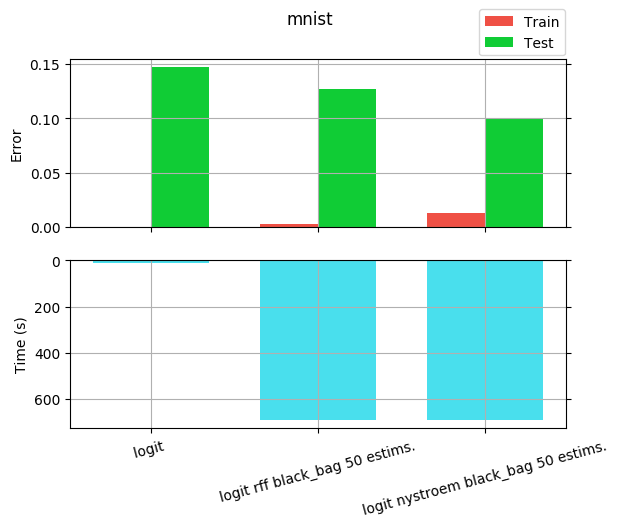
\includegraphics[scale=\imgscale]{Figures/2_2/mnist}
\decoRule
\caption[2.2 mnist]{Logistic Regression with Black Bag model}
\label{fig:2_2_mnist}
\end{figure}

\begin{figure}[th]
\centering
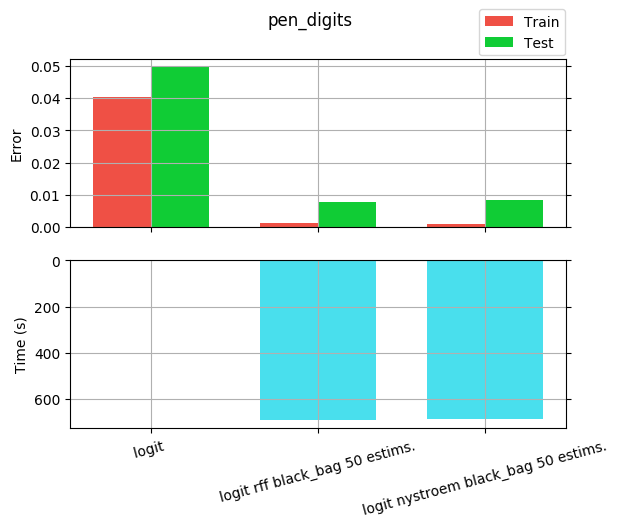
\includegraphics[scale=\imgscale]{Figures/2_2/pen_digits}
\decoRule
\caption[2.2 pen\tu digits]{Logistic Regression with Black Bag model}
\label{fig:2_2_pen_digits}
\end{figure}

\begin{figure}[th]
\centering
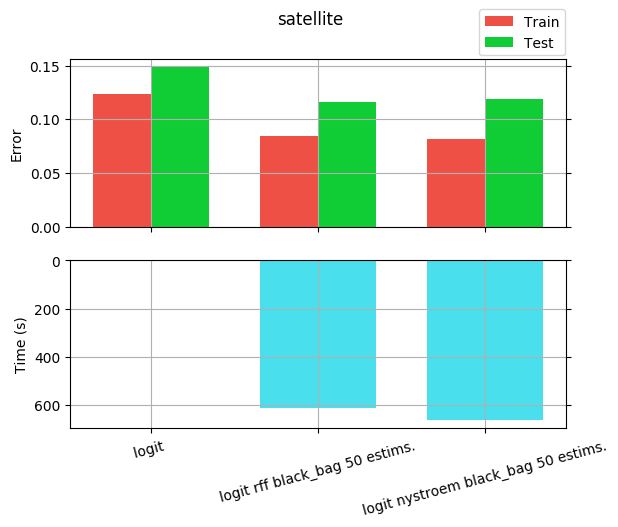
\includegraphics[scale=\imgscale]{Figures/2_2/satellite}
\decoRule
\caption[2.2 satellite]{Logistic Regression with Black Bag model}
\label{fig:2_2_satellite}
\end{figure}

\begin{figure}[th]
\centering
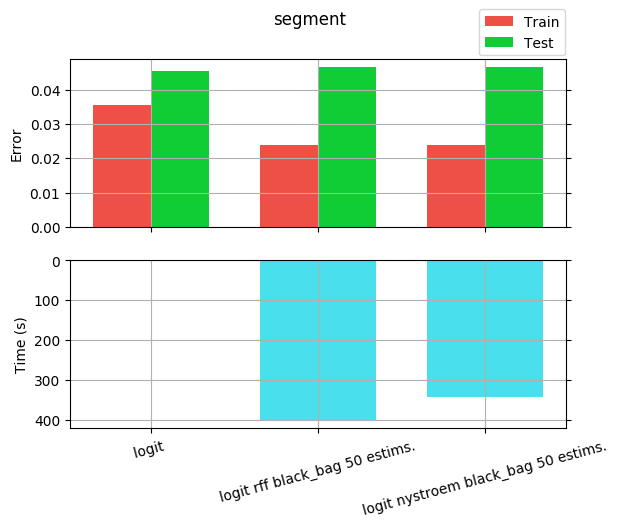
\includegraphics[scale=\imgscale]{Figures/2_2/segment}
\decoRule
\caption[2.2 segment]{Logistic Regression with Black Bag model}
\label{fig:2_2_segment}
\end{figure}

\begin{figure}[th]
\centering
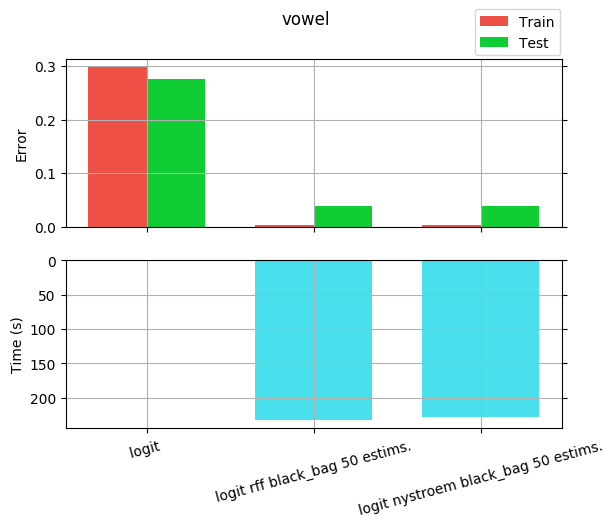
\includegraphics[scale=\imgscale]{Figures/2_2/vowel}
\decoRule
\caption[2.2 vowel]{Logistic Regression with Black Bag model}
\label{fig:vowel}
\end{figure}
